\documentclass[conference]{IEEEtran}
\IEEEoverridecommandlockouts
\usepackage{cite}
\usepackage[utf8]{inputenc}
\usepackage[english]{babel}
\usepackage{bookmark}
\usepackage[square,sort,comma,numbers]{natbib}
\usepackage{listings}
\usepackage{url}
\usepackage{wrapfig}
\usepackage{caption}
\usepackage{color}
\usepackage{enumitem}
\usepackage{graphicx}
\usepackage{float}
\usepackage{url}
\def\UrlBreaks{\do\/\do-}
\usepackage{breakurl}
\graphicspath{{images/}}
\usepackage{hyperref}

\def\BibTeX{{\rm B\kern-.05em{\sc i\kern-.025em b}\kern-.08em
T\kern-.1667em\lower.7ex\hbox{E}\kern-.125emX}}


\begin{document}

\title{Crime Prediction using Deep Learning\\[0.3cm]
\large Final Report\\
ELE494-09}


\author{
\IEEEauthorblockN{Nasir Khalid}
\IEEEauthorblockA{b00065082}
\and
\IEEEauthorblockN{Yousif Khaireddin}
\IEEEauthorblockA{b00063618}
}

\maketitle

\begin{abstract}
The following report details our attempt to predict crime in the city of Vancouver using deep
neural networks. It starts by explaining the need for crime prediction and its challenges. We then talk about some of the previous work that researchers have done to predict crime
and then we highlight what we have done differently in our networks. The report also discusses all of the
data used and all the data preprocessing that was done to produce our final datasets. We then discuss the
4 different networks we trained highlighting their inputs, outputs, architectures, training and test results.
We conclude with a closing remark on how our networks could be improved and what can be done for actual prediction.
\end{abstract}

\IEEEpeerreviewmaketitle


\section{Introduction}

Around the world police departments from different regions invest large amounts
of money in finding ways to discover crime trends, uncover potential crime plans and
develop better policing techniques. In the early days of crime prediction and technology,
this was mainly done by observing historical data to find common trends in crime over years,
months or even days. Apart from this a lot of undercover officers were used to patrol and be on
the lookout for suspicious ongoings in the city. These methods were often very expensive and ignored
certain factors that affect crime.\\

Crime itself is unpredictable in nature when viewed on its own and it is shown to be dependent
on various different factors such as weather, location, social and economic factors \cite{Carlen}
When prediction was done using historical data these factors were ignored and therefore the models
did not perform well. With the advancement of deep learning and high powered computers a new method of
crime prediction became more viable, a method that was capable of finding links between various other factors and crime.
However, crime prediction is a field that has not received the same level of attention from deep learning as other fields
like computer vision, generative modeling etc.\\

Deep neural networks are designed to reduce the need for extensive feature engineering and allow for training over large datasets.
The deep entanglement of crime, multiple variables and it's dependency on spatial and temporal factors (location and time of day)
make it an ideal candidate for prediction with a deep neural network.

\section{Literature Review}

One of the earliest cases of crime prediction through a neural network used regression to predict the monthly
911 calls and thereby predict crime \cite{olligschlaegerartificial}. However, this network was limited by technology and 
was not capable of using location and other factors for prediction. \\

Another recent method was to divide the city in to a grid like a checkerboard and data is aggregated within each cell. These
cells also contain previous days crime as well as information about the neighboring cell, this was used to then predict the average
number of crimes over a month and the type of crimes within a month \cite{6137459}\\

The most recent paper on this topic \cite{stec2018forecasting} once again used a grid like division of the city like the one in \cite{6137459} however they instead used
a RNN and CNN to train the network to account for temporal and spatial information instead of adding crime data from previous days and 
using the neighboring cell data. 

\section{Method}

For our project we wanted to step away from the methods used in \cite{stec2018forecasting} and \cite{6137459} that relied on splitting a city in to cells
and training networks only on these cells. Instead we wanted to utilize the existing location details available in many datasets such as co-ordinates and neighbourhoods to
predict crime. To do this we created multiple different networks that all utilized data that was available in our datasets and did not need divisions of a city in to
grid blocks.

\subsection{Datasets Used}

For the project we obtained all of our data from the city of Vancouver’s open data source \cite{data}. Listed below are all the datasets
we used in our project, their specific use cases are discussed in detail in further sections.\\

\subsubsection{Crime Data}

~\\The first dataset we obtained from the website was the crime dataset \cite{crime}. The columns of the dataset were the following:\\

\begin{itemize}
  \item Type of crime
  \item Year
  \item Day
  \item Month
  \item Hour
  \item Minute
  \item Block of crime
  \item Neighbourhood of crime
  \item X Co-ordinate of crime in UTM Zone 10
  \item Y Co-ordinate of crime in UTM Zone 10
  \item Latitude
  \item Longitude\\
\end{itemize}

The entire dataset consisted of 530652 crimes from 2003 to 2017. However, for some of the them their time
and location data was missing as it was protected for privacy reasons. This data was essentially useless for us so we eliminated
all of these crimes and that left us with a total of 476290 crimes to work with.\\

Shown below is a figure showing the number of crimes per day from 2004 to 2017 obtained from the dataset:

\begin{figure}[H]
  \centering
  \captionsetup{justification=centering}
  \centering
  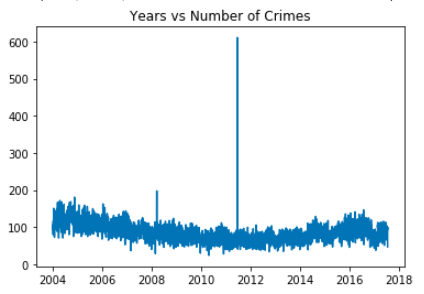
\includegraphics[width=2.5in]{2.png}
  \caption{Crimes per day from 2004 to 2017}  
  \label{1}
\end{figure}

\subsubsection{Neighbourhood Dataset}

~\\We then downloaded a second dataset from the Vancouver open data catalogue that gave us a list of neighborhoods in Vancouver \cite{nb}.
We added 2 new columns to this dataset called ’Latitude’ and ’Longitude’ and in here we added the center
latitude and longitude for each respective neighborhood. This second dataset consisted of the following\\
columns:\\

\begin{itemize}
  \item Map ID
  \item Neighbourhood Name
  \item Neighbourhood Center Latitude (Added)
  \item Neighbourhood Center Longitude (Added)\\
\end{itemize}

\subsubsection{Graffiti Dataset}

~\\A list of 8508 points detailing the exact location of all known graffiti in Vancouver \cite{graffiti}. The dataset has the
following columns:\\

\begin{itemize}
  \item Latitude 
  \item Longitude\\
\end{itemize}

\subsubsection{Water Fountain Dataset}

~\\A list of 241 drinking fountains scattered around Vancouver \cite{fountain} containing specific information about each of them, the dataset has the following
columns:\\

\begin{itemize}
  \item Map ID 
  \item Latitude
  \item Longitude
  \item Name
  \item Location
  \item Maintainer
  \item In Operation
  \item Pet Friendly
  \item Photo\\
\end{itemize}

For our project we only rely on the latitude and longitude information from the dataset, the other columns are discarded.\\

\subsubsection{Google Search Trends of Crime}

~\\A monthly index describing the rate at which the word “crime” has been searched throughout a month relative
to that of the maximum month \cite{Google}. This dataset spans from 2004 till present, so it requires the removal of 1 year
of the crime data (2003) during merging.\\

We use this dataset because during our research we learned that there is a very high
correlation between the 6-Months Moving Average moving average of google searches for crime and the
6-Months Moving Average of crimes in Vancouver, this can be seen in the figure below:

\begin{figure}[H]
  \centering
  \captionsetup{justification=centering}
  \centering
  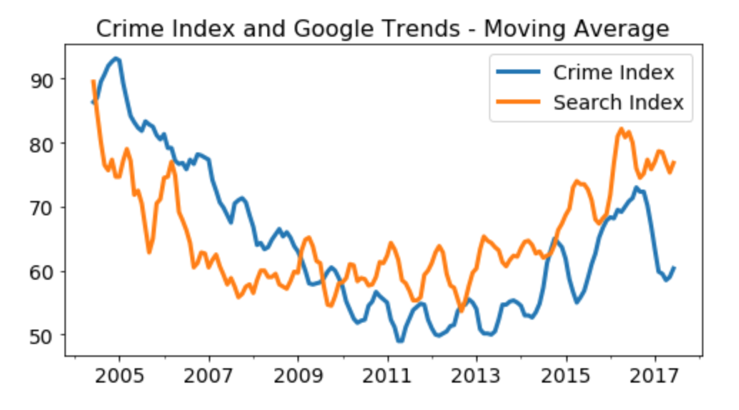
\includegraphics[width=2.7in]{3.png}
  \caption{ 6 Month moving average of Crime and Crime Search}  
  \label{3}
\end{figure}

We decided to include this metric of google searches into our final dataset. We decided that for each datapoint, we would insert the google crime search trend of the previous month,
and the code for including this to the final dataset can be found on the project repository. \cite{Trend_Script}
One important thing to notice is that this is a form of temporal dependency since it is indirectly describing the behaviors of
this dataset for each entry over time.

\subsection{Final Dataset}

It is important to note that all the previously listed datasets waere then further filtered and manipulated to fit
the needs of each and every network we built, and this will be discussed in the respective network sections.
Some networks utilized more datasets than others, and this was dependent on the nature of the problem at hand,
as will be described later. However, we did compile all available data and create a final crime dataset \cite{finalcrime} that was imported
to each networks respective Jupyter notebook. It consists of the following columns:\\

\begin{itemize}
  \item Type of Crime 
  \item Year
  \item Month
  \item Day
  \item Hour
  \item Minute
  \item Latitude
  \item Longitude
  \item Neighbourhood
  \item Block of Crime
  \item X Co-ordinate of crime in UTM Zone 10
  \item Y Co-ordinate of crime in UTM Zone 10
  \item Distance from nearest Graffiti
  \item Distance from nearest Drinking Fountain
  \item Google Trend Data for previous month\\
\end{itemize}

\subsubsection{Distance from nearest Graffiti and Drinking Fountain}

~\\These columns in the final dataset were added manually by us. We first looped over all crimes and for each crime we calculated its distance in kilometres
from each of the different graffiti locations and each of the different drinking fountain locations. We then got the smallest value for each calculated
distance and added it to the dataset. This was done to account for spatial features that consider the presence of nearby factors that could lead to crime.
The script used for this process can be found on the project repository \cite{Crime_Extractor} \cite{Drinking_Fountain_Extractor}

Shown below is a histogram of the distances from crimes and it is clear that crimes happen frequently near graffiti and around a certain distance away from
drinking fountains.

\begin{figure}[H]
  \centering
  \captionsetup{justification=centering}
  \centering
  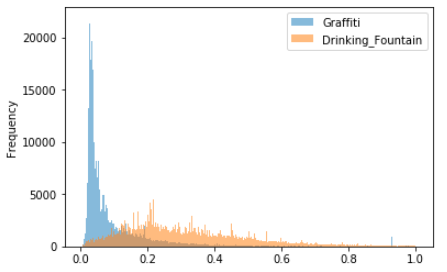
\includegraphics[width=2.5in]{1.png}
  \caption{Histogram of Distance from Graffiti and Distance from Drinking Fountain}  
  \label{1}
\end{figure}

\subsection{Training Plan}

Now that we had collected our dataset with multiple different variables our plan was to create multiple different networks with different variations and see
the results that we obtain from each of these networks. We trained various deep neural networks and these are outlined in the upcoming sections.

\section{Experiments}

\subsection{Network 1 \cite{Network_1}}

For one of our very first networks, we decided to create a sum of total crimes per neighborhood per day.
This can be done by first up-sampling the crime dataset to include all neighborhoods in each day even if there was no crime in the neighborhood,
then we sum the number of crimes per day per neighborhood. So per day there are 22 entries (one for each neighborhood) and there is a new column with the
total number of crimes. A graph of this can be seen below:

\begin{figure}[H]
  \centering
  \captionsetup{justification=centering}
  \centering
  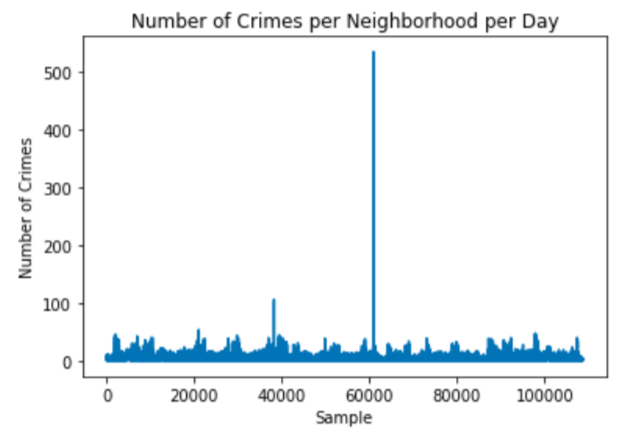
\includegraphics[width=2.5in]{4.png}
  \caption{Number of Crimes per Neighbourhood per day}  
  \label{1}
\end{figure}

Once the above has been completed, we can then pool these different crimes into bins which denote a range of crimes.
This is important as it will enable us to easily one hot encode the crime values into a number of classes.
This is useful as it reduces the complexity of the problem. For our application, we chose the following ranges:\\

\begin{itemize}
  \item Class 0: 0 – 1 crimes
  \item Class 1: 2 - 3 crimes
  \item Class 2: 4 - 5 crimes
  \item Class 3: Greater than 5 crimes\\
\end{itemize}

A graph displaying this information can be seen below:

\begin{figure}[H]
  \centering
  \captionsetup{justification=centering}
  \centering
  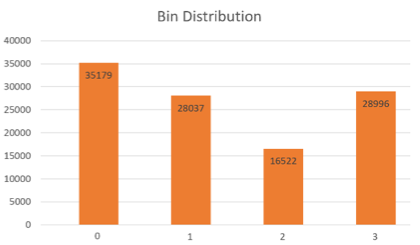
\includegraphics[width=2.5in]{5.png}
  \caption{Bin Distribution}  
  \label{1}
\end{figure}

All of this was compiled in to a dataset that is available on the project repository \cite{bins} and the code used to perform
this is also available \cite{bin_code}

Once this data has been formulated, we can then run this information through a neural network.
For this task, we decided to build a simple feedforward network since there is no clear method to map this information
into a CNN or RNN.

The network inputs:

\begin{itemize}
  \item Year
  \item Month
  \item Day
  \item Neighbourhood\\
\end{itemize}

The network output:

\begin{itemize}
  \item A vector with a probability associated to each bin\\
\end{itemize}

We used the following network architecture which had the best performance:

\begin{figure}[H]
  \centering
  \captionsetup{justification=centering}
  \centering
  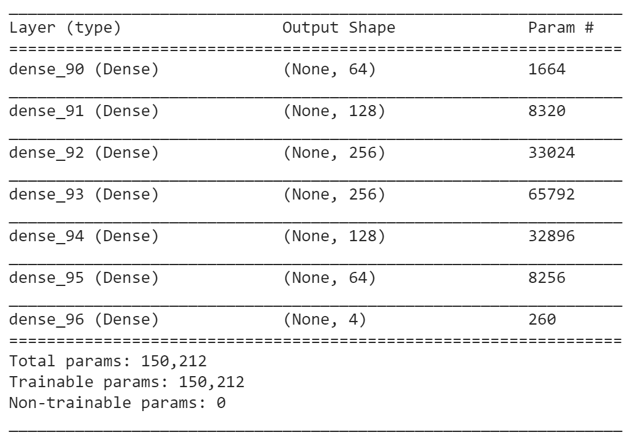
\includegraphics[width=2.5in]{6.png}
  \caption{Network 1 Architecture}  
  \label{1}
\end{figure}

The following two plots show the accuracy and loss of our network throughout the training:

\begin{figure}[H]
  \centering
  \captionsetup{justification=centering}
  \centering
  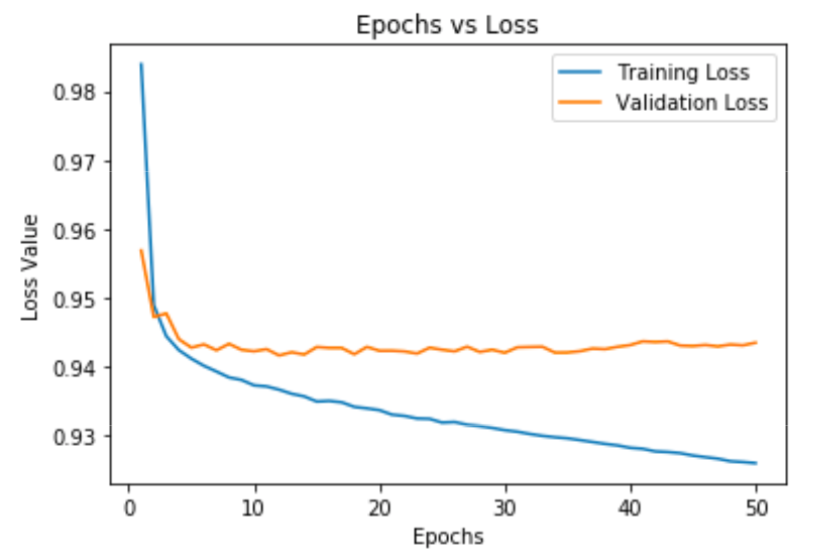
\includegraphics[width=2.5in]{7.png}
  \caption{Network 1: Epoch vs Loss}  
  \label{1}
\end{figure}

\begin{figure}[H]
  \centering
  \captionsetup{justification=centering}
  \centering
  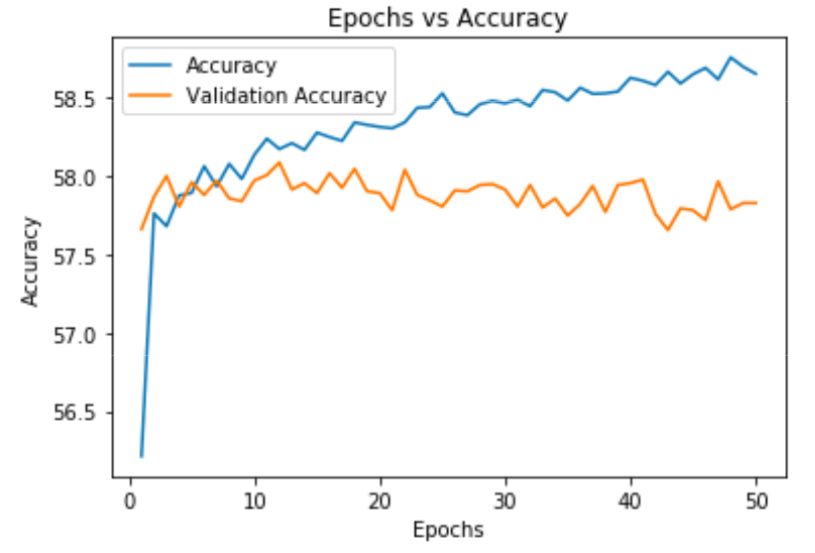
\includegraphics[width=2.5in]{8.png}
  \caption{Network 1: Epoch vs Accuracy}  
  \label{1}
\end{figure}

When used on the test data, the network had a final test loss of 0.97219 and an accuracy of 58\%. The confusion matrix is
shown below:

\begin{figure}[H]
  \centering
  \captionsetup{justification=centering}
  \centering
  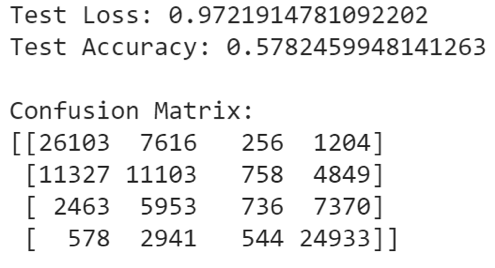
\includegraphics[width=2.5in]{9.png}
  \caption{Network 1: Confusion Matrix}  
  \label{1}
\end{figure}

The network above is not ideal by any means; however, it is important to note that increasing the complexity
of the network did not yield any better results. Next, it is important to note that since we are not overfitting
the data, we did not put any means of regularization or dropout, as was seen in the network architecture above.
This, however, does show that it might be possible to properly predict the number of crimes per neighborhood
per day should we have a larger dataset, or some more features on this data.


\subsection{Network 2 \cite{Network_2}}

In this network we attempted to predict the type of crime that was most likely at a certain hour of day
in a certain location. For this network we used the previously mentioned final dataset that we had prepared \cite{finalcrime}
as it contains all the needed data. 

The network inputs:

\begin{itemize}
  \item Year
  \item Month
  \item Day
  \item Latitude
  \item Longitude
  \item Distance to Graffiti
  \item Distance to a Drinking Fountain
\end{itemize}

The network output:

\begin{itemize}
  \item A vector with a probability associated to each Type of Crime\\
\end{itemize}

The required columns were imported and the output was a one hot encoded vector related to each crime. Before training we also
tried to understand which crimes happen most frequently as we understand that our network would return a higher probability related
to those ones. Shown below is a histogram of the dataset showing the count for different types of crimes:

\begin{figure}[H]
  \centering
  \captionsetup{justification=centering}
  \centering
  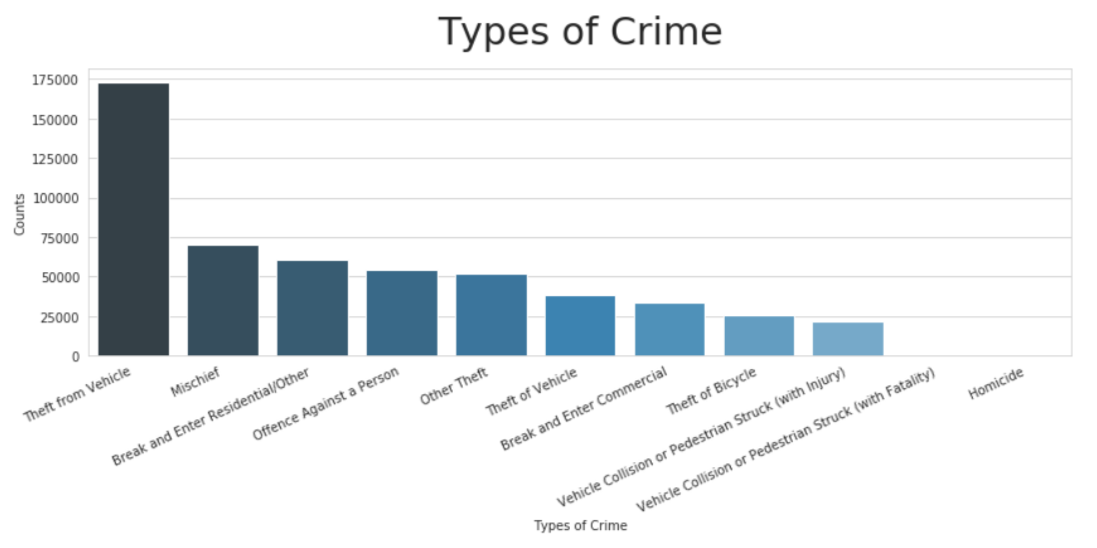
\includegraphics[width=2.5in]{10.png}
  \caption{Histogram of types of Crime in city}  
  \label{1}
\end{figure}

We used the following network architecture which had the best performance:

\begin{figure}[H]
  \centering
  \captionsetup{justification=centering}
  \centering
  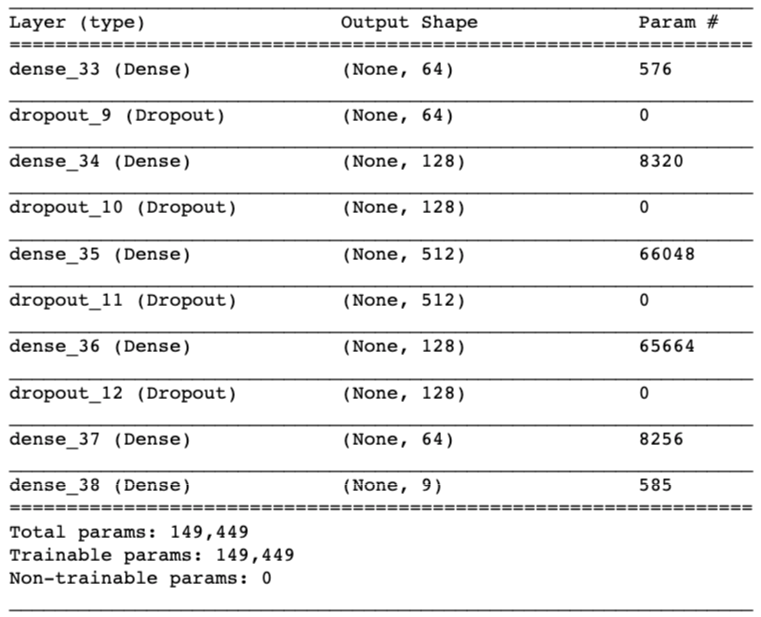
\includegraphics[width=2.5in]{11.png}
  \caption{Network 2 Architecture}  
  \label{1}
\end{figure}

The following two plots show the accuracy and loss of our network throughout the training:

\begin{figure}[H]
  \centering
  \captionsetup{justification=centering}
  \centering
  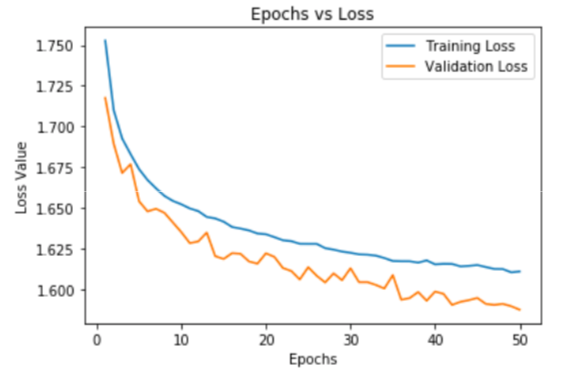
\includegraphics[width=2.5in]{12.png}
  \caption{Network 2: Epoch vs Loss}  
  \label{1}
\end{figure}

\begin{figure}[H]
  \centering
  \captionsetup{justification=centering}
  \centering
  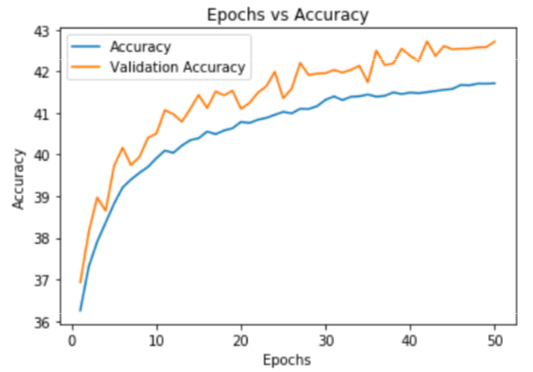
\includegraphics[width=2.5in]{13.png}
  \caption{Network 2: Epoch vs Accuracy}  
  \label{1}
\end{figure}

On the test set the network had a 43\% accuracy. Although our network did not perform well in terms of accuracy we still found
that it had some sort of understanding in to the occurance of crime and times of day at a certain location. For example as we
see the output of the network over 24 hours we see that it shows a lower chance of crime due to vehicle/pedestrain accident at night
but more during rush hour. This does make sense and it shows that there is some understanding that our network is able to develop
during training phase. There may be more cases like which are not explicitly visible at first glance. Shown below is an image displaying
the results over 24 hours and the probability changing over time:

\begin{figure}[H]
  \centering
  \captionsetup{justification=centering}
  \centering
  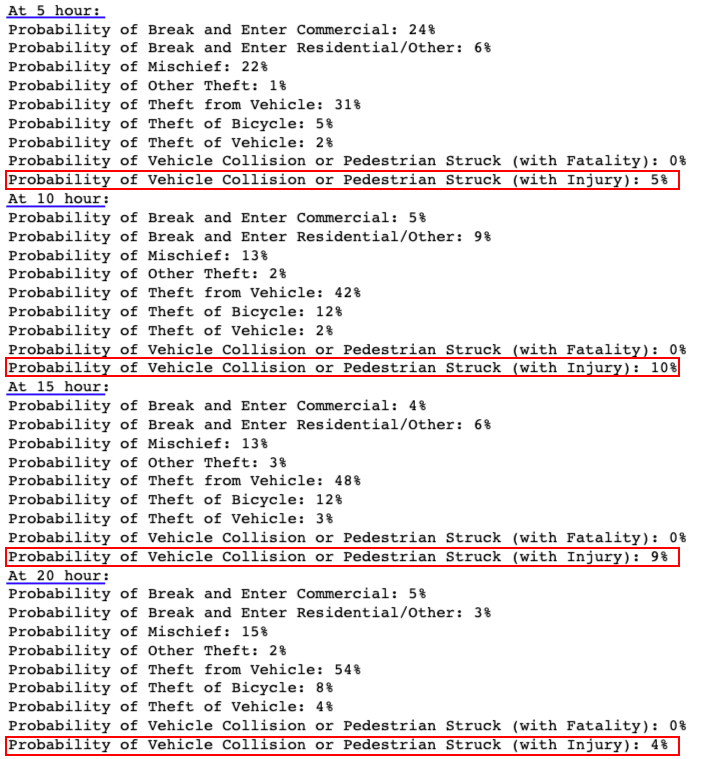
\includegraphics[width=3in]{14.png}
  \caption{Network 2: Result over 24 hours with pedestrian/vehicle collision highlighted}  
  \label{1}
\end{figure}

\subsection{Network 3 \cite{Network_3}}

In this network we attempted to predict the probability of crime in a neighborhood at a certain hour of day.
For this network we used the previously mentioned final dataset that we had prepared \cite{finalcrime}
as it contains all the needed data. 

The network inputs:

\begin{itemize}
  \item Year
  \item Month
  \item Day
  \item Hour
  \item Neighbourhood (One hot encoded)
\end{itemize}

The network output:

\begin{itemize}
  \item Probability of crime occuring\\
\end{itemize}

Here before training the data was first given a 'Crime' column with a value of 1 indicating that a crime happened. Then
we performed upsampling. The data is upsampled by neighborhood so that if for some day/time there was no crime in a neighborhood,
a point was added for that neighborhood and the 'Crime' column value was set to 0. We also upsampled by 1 hour so that if there was
no crime at for example 6:00 am in a neighborhood, a row was added for that time and neighborhood with it's 'Crime' value set to 0.

We used the following network architecture which had the best performance:

\begin{figure}[H]
  \centering
  \captionsetup{justification=centering}
  \centering
  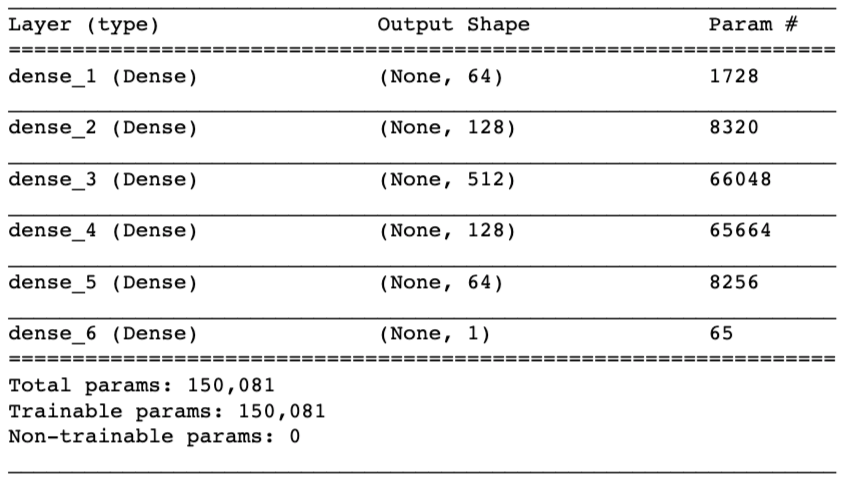
\includegraphics[width=2.5in]{15.png}
  \caption{Network 3 Architecture}  
  \label{1}
\end{figure}

The following two plots show the accuracy and loss of our network throughout the training:

\begin{figure}[H]
  \centering
  \captionsetup{justification=centering}
  \centering
  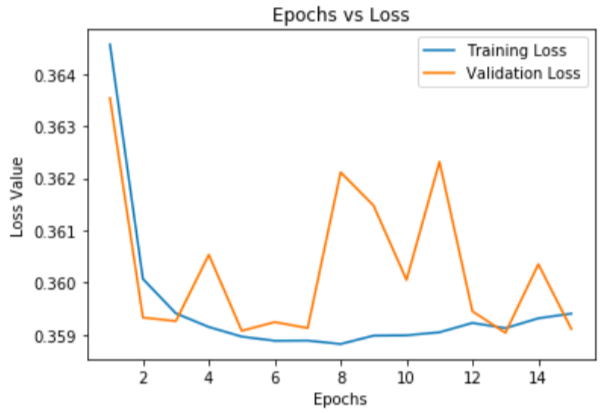
\includegraphics[width=2.5in]{16.png}
  \caption{Network 3: Epoch vs Loss}  
  \label{1}
\end{figure}

\begin{figure}[H]
  \centering
  \captionsetup{justification=centering}
  \centering
  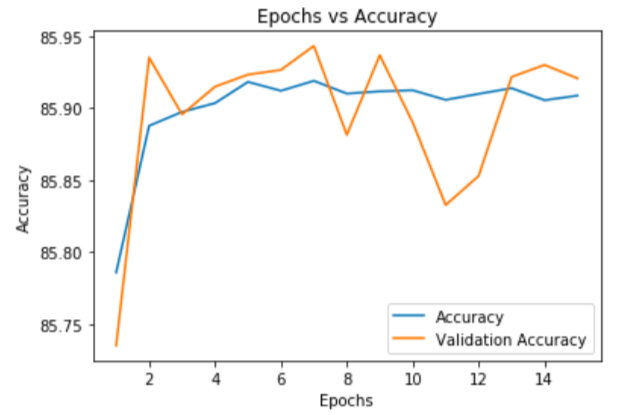
\includegraphics[width=2.5in]{17.png}
  \caption{Network 3: Epoch vs Accuracy}  
  \label{1}
\end{figure}

On the test dataset the network had a final loss of 0.36 and an accuracy of 86\%. The output for a given day and location over 24 hours is
shown below and it does exhibit a logical pattern with crime being more likely to happen at night but not very likely around the early hours:

\begin{figure}[H]
  \centering
  \captionsetup{justification=centering}
  \centering
  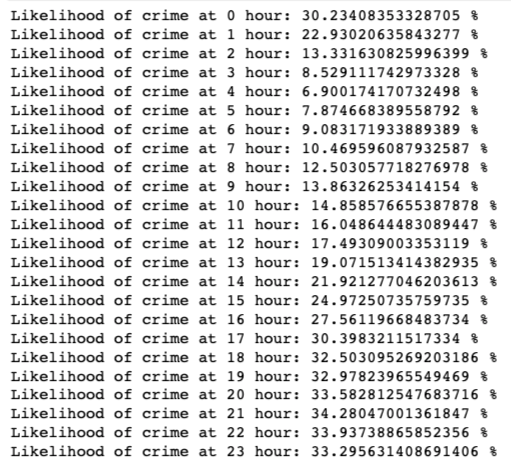
\includegraphics[width=1.6in]{18.png}
  \caption{Network 3: Prediction Output}  
  \label{1}
\end{figure}

\subsection{Network 3.1 \cite{Network_3.1}}

Network 3.1 was retrained to give the same output as Network 3 but the inputs to the network were changed to be the following:

\begin{itemize}
  \item Year
  \item Month
  \item Day
  \item Hour
  \item Minute
  \item Latitude
  \item Longitude
  \item Distance from nearest Graffiti
  \item Distance from nearest Drinking Fountain
\end{itemize}

he following two plots show the accuracy and loss of our network throughout the training:

\begin{figure}[H]
  \centering
  \captionsetup{justification=centering}
  \centering
  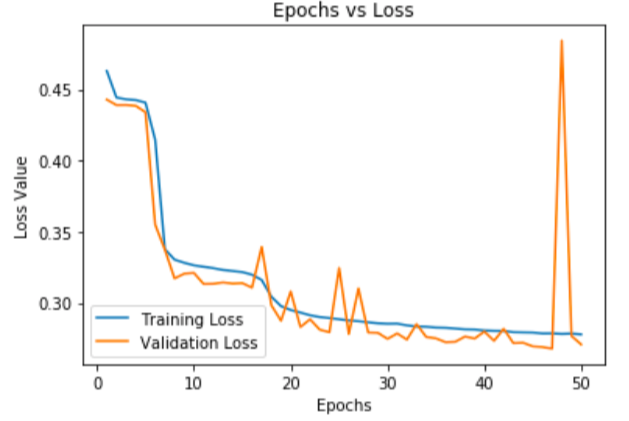
\includegraphics[width=2.5in]{19.png}
  \caption{Network 3.1: Epoch vs Loss}  
  \label{1}
\end{figure}

\begin{figure}[H]
  \centering
  \captionsetup{justification=centering}
  \centering
  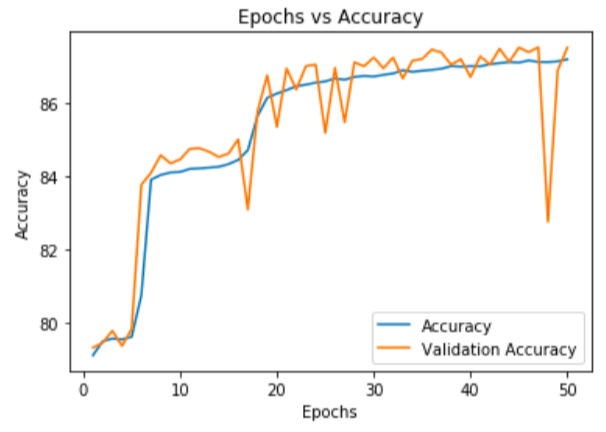
\includegraphics[width=2.5in]{20.png}
  \caption{Network 3.1: Epoch vs Accuracy}  
  \label{1}
\end{figure}

Although this network has a test accuracy of 87.23\%. The prediction output gives a near 100\% chance of crime throughout the day/hour no
matter what the input \cite{Network_3.1}.

\subsection{Network 3.2 \cite{Network_3.2}}

Network 3.2 was retrained to give the same output as Network 3 but the inputs to the network were changed to be the following:

\begin{itemize}
  \item Year
  \item Month
  \item Day
  \item Hour
  \item Minute
  \item Latitude
  \item Longitude
  \item Distance from nearest Graffiti
  \item Distance from nearest Drinking Fountain
  \item Google Trend Data
\end{itemize}

The following two plots show the accuracy and loss of our network throughout the training:

\begin{figure}[H]
  \centering
  \captionsetup{justification=centering}
  \centering
  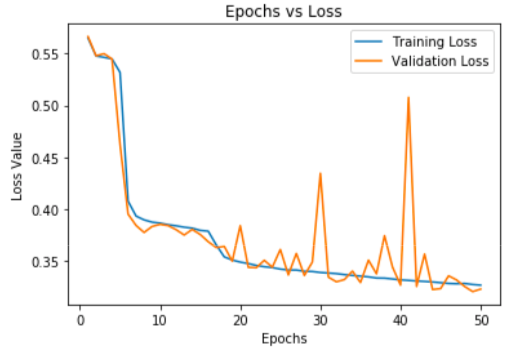
\includegraphics[width=2.5in]{21.png}
  \caption{Network 3.2: Epoch vs Loss}  
  \label{1}
\end{figure}

\begin{figure}[H]
  \centering
  \captionsetup{justification=centering}
  \centering
  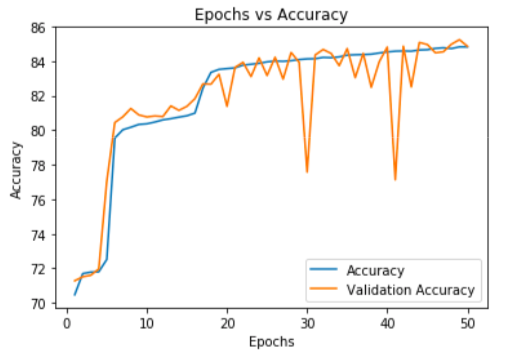
\includegraphics[width=2.5in]{22.png}
  \caption{Network 3.2: Epoch vs Accuracy}  
  \label{1}
\end{figure}

Although this network has a test accuracy of 84.69\%. The prediction output gives a better output than Network 3.1 which therefore
means that the Google Trend data does have an effect on the network's ability to succeed. \cite{Network_3.2}.

\subsection{Network 4 \cite{Network_4}}

Here we attempted to predict which neighborhoods would have crime given the year, month, day and hour. This was done in a similar
style to a multi-class classification where each neighborhood was a class and the network was trained to output the multiple
classes where a crime would happen for a give year, month and day.

We used the following network architecture which had the best performance:

\begin{figure}[H]
  \centering
  \captionsetup{justification=centering}
  \centering
  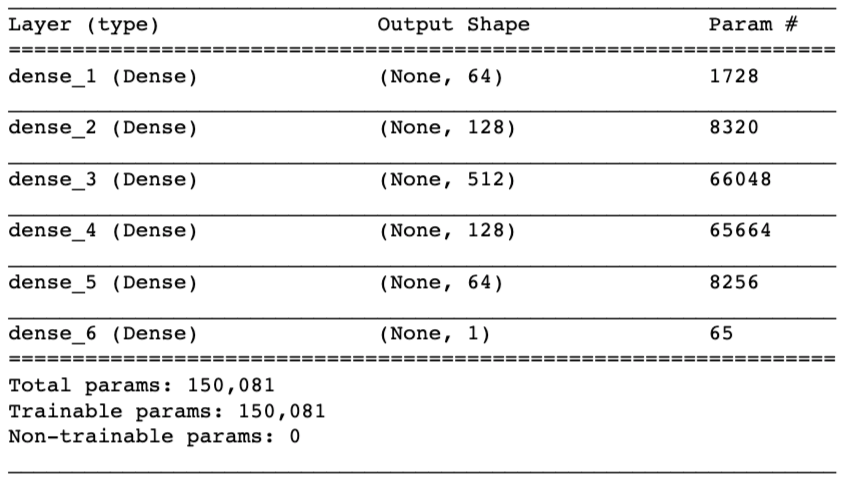
\includegraphics[width=2.5in]{15.png}
  \caption{Network 4 Architecture}  
  \label{1}
\end{figure}

The following two plots show the accuracy and loss of our network throughout the training:

\begin{figure}[H]
  \centering
  \captionsetup{justification=centering}
  \centering
  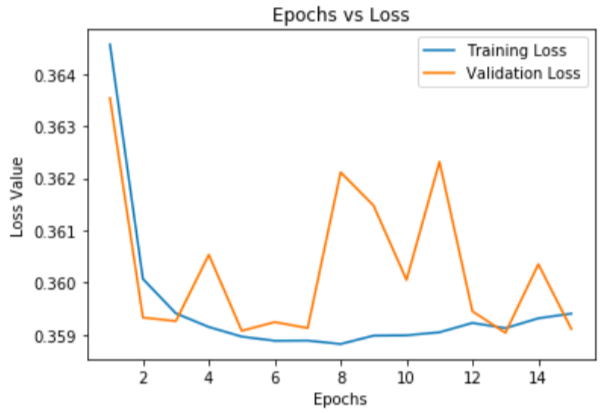
\includegraphics[width=2.5in]{16.png}
  \caption{Network 4: Epoch vs Loss}  
  \label{1}
\end{figure}

\begin{figure}[H]
  \centering
  \captionsetup{justification=centering}
  \centering
  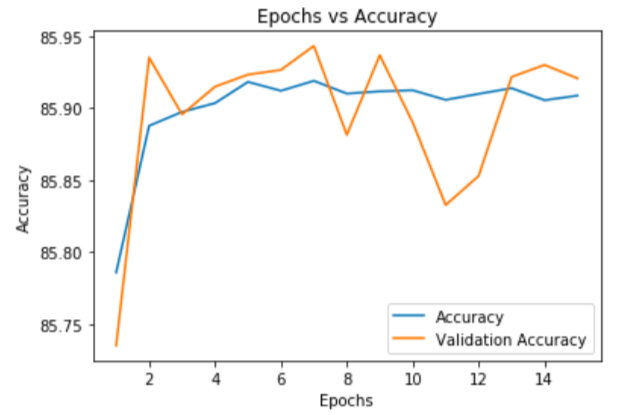
\includegraphics[width=2.5in]{17.png}
  \caption{Network 4: Epoch vs Accuracy}  
  \label{1}
\end{figure}

On the test dataset we had an accuracy of 86.15\%. 

\section{Conclusion}

Predicting crime is no easy task due to its dependency on multiple factors, through our different experiments we were able to produce
networks that found various different patterns in crime and used them to improve prediction results. We do believe that having a larger
dataset could lead to further improvements in our network. Furthermore, certain factors like weather which we wanted to incorporate in
our dataset were not available and using them alongside the other variables we introduced could lead to even better results. 

We also believe that using multiple networks together is the way forward. Such as using network 2 and 4 to predict where crime will happen
and what time of crime will occur.

\bibliographystyle{IEEEtran}
\bibliography{report}

\end{document}